% =============================================================================
% practica7.tex --- Chapter: Practice 7
% =============================================================================

\documentclass[../../__memoria.tex]{subfiles}

\begin{document}
\standalonecover
\pagestyle{cuerpo}

\chapter[Práctica 7: Modelos de Ensambles]{Cuaderno de Laboratorio --- Práctica 7: La Inteligencia Colectiva (Modelos de Ensambles)}

\section*{Introducción}
En esta práctica usamos el dataset \textit{Breast Cancer Wisconsin}, que recoge medidas extraídas de imágenes de biopsias mamarias para clasificar tumores entre benignos y malignos. Lo interesante de esta práctica es que no solo entrenamos modelos, sino que los comparamos entre sí para entender cuándo complejidad es ganancia real y cuándo es simplemente sobreajuste disfrazado.

% -----------------------------------------------------------------------------
\section[Tarea 1: Árbol Solitario]{Tarea 1 --- Árbol Solitario (Baseline)}
% -----------------------------------------------------------------------------

Como punto de partida, entrenamos un Árbol de Decisión sin ningún límite de profundidad (\mbox{\texttt{max\_depth=None}}) para establecer un \textit{baseline}.

\textbf{Resultados:}
\begin{itemize}
    \item \textit{Accuracy} en entrenamiento: 1.0000
    \item \textit{Accuracy} en test: 0.9231
\end{itemize}

\textbf{Sobreajuste:}
Un 100\% en entrenamiento y un 92.3\% en test es una señal bastante clara de sobreajuste. Sin límite de profundidad, el árbol no para de dividirse hasta que cada hoja tiene exactamente una muestra. Esto significa que el espacio de entrada queda troceado en regiones tan pequeñas que cada muestra de entrenamiento tiene prácticamente su propia cajita. Cuando llega un dato nuevo, lo más probable es que caiga en una región diseñada a medida para otra muestra concreta del entrenamiento, y el modelo no sepa qué hacer con él.

El problema de fondo es la sensibilidad al ruido: cualquier valor ligeramente raro por un error de medición o simplemente por variación natural hace que el árbol construya una rama entera solo para ese caso. Esas ramas no generalizan nada, solo sirven para ese punto concreto. El resultado es que el árbol ``aprende'' también los errores y las casualidades del entrenamiento, no solo el patrón real.

% -----------------------------------------------------------------------------
\section[Tarea 2: Random Forest]{Tarea 2 --- Bagging y Random Forest}
% -----------------------------------------------------------------------------

Para atacar el sobreajuste del árbol simple, probamos Random Forest, que aplica la estrategia de \textit{Bagging}: en lugar de un solo árbol con todos los datos, entrenas muchos árboles distintos y dejas que voten.

\begin{center}
  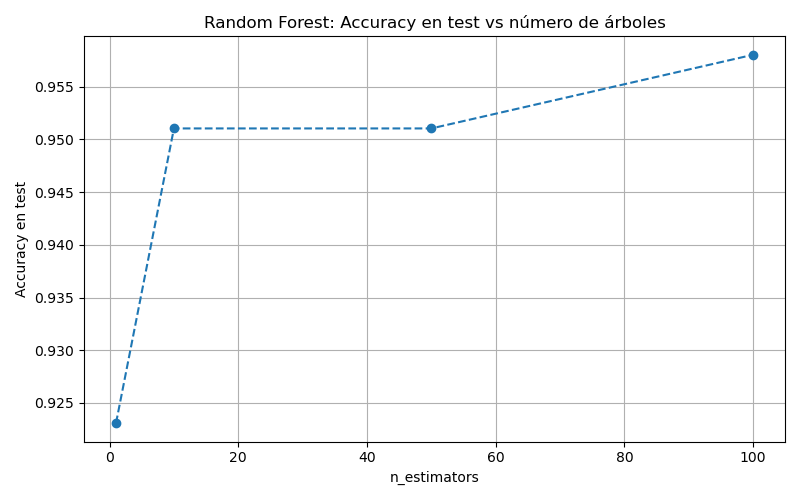
\includegraphics[width=0.85\linewidth]{img/rf_accuracy.png}
\end{center}

\textbf{Análisis:}
La gráfica muestra cómo el \textit{accuracy} en test sube de 0.923 con un árbol a 0.958 con 100. La clave está en el \textit{bootstrapping}: para cada árbol se crea un subconjunto de los datos tomando muestras con reemplazo, lo que significa que una misma muestra puede repetirse y otras pueden no aparecer. Así cada árbol ve una versión ligeramente distinta del dataset y aprende cosas un poco diferentes.

Al combinar sus predicciones por votación, los errores individuales de cada árbol tienden a cancelarse. Matemáticamente, al promediar $M$ modelos independientes, la varianza del conjunto resultante es aproximadamente $\frac{1}{M}$ de la suma de las varianzas de cada uno. Por eso esta técnica reduce el error sin aumentar el sesgo: cada árbol sigue siendo tan profundo y expresivo como antes (sesgo bajo), pero al juntarlos se suavizan los errores aleatorios que cada uno cometería por separado.

A partir de los 50 árboles la curva se aplana (entre 0.951 y 0.958). Llegado a ese punto, añadir más árboles no aporta diversidad nueva a la votación porque el conjunto ya ha capturado prácticamente toda la información disponible.

% -----------------------------------------------------------------------------
\section[Tarea 3: Boosting]{Tarea 3 --- El poder del Boosting}
% -----------------------------------------------------------------------------

El tercer modelo que probamos fue Gradient Boosting, cuya filosofía es bastante diferente a la de Random Forest.

\textbf{Random Forest vs.\ Gradient Boosting:}
Random Forest construye todos sus árboles de forma independiente, lo que permite paralelizarlos sin problema. Gradient Boosting, en cambio, los entrena en secuencia: cada árbol nuevo intenta corregir los errores del anterior, ajustándose al gradiente de la función de pérdida. Es un proceso mucho más iterativo y dirigido.

\textbf{Rendimiento y Coste:}
\begin{itemize}
    \item \textit{Accuracy} en test: 0.9580
    \item Tiempo de entrenamiento: $\approx$ 0.2512 s (frente a $\approx$ 0.2103 s de Random Forest con 100 árboles).
\end{itemize}
Los dos modelos alcanzan el mismo 95.8\% de \textit{accuracy}, pero Gradient Boosting tarda algo más (unos 0.04 s en esta ejecución). En un dataset tan pequeño la diferencia es casi anecdótica, pero en datasets más grandes la naturaleza secuencial del boosting empieza a pesar de verdad porque no puedes distribuir el trabajo entre núcleos de la misma forma.

\textbf{Importancia de Variables:}
Las tres características que más influyeron en las predicciones del modelo fueron:
\begin{enumerate}
    \item \texttt{worst radius} (importancia: $\approx$ 55.9\%)
    \item \texttt{worst concave points} (importancia: $\approx$ 13.2\%)
    \item \texttt{worst perimeter} (importancia: $\approx$ 12.8\%)
\end{enumerate}

Tiene mucho sentido desde el punto de vista clínico: las células malignas tienden a tener núcleos más grandes e irregulares que las benignas. El radio, el perímetro y los puntos cóncavos del contorno son justamente las medidas que capturan esa deformación estructural. Que el modelo les asigne tanto peso indica que está usando la misma lógica que usaría un médico mirando una imagen: ¿el núcleo es grande y deforme?

% -----------------------------------------------------------------------------
\section[Comparación y Reflexión]{Tarea 4 --- Comparación Global y Reflexión}
% -----------------------------------------------------------------------------

\begin{table}[H]
    \centering
    \resizebox{\textwidth}{!}{%
    \begin{tabular}{|l|c|c|p{5cm}|p{5cm}|}
    \hline
    \textbf{Modelo} & \textbf{Acc. Test} & \textbf{Coste} & \textbf{Ventajas} & \textbf{Desventajas} \\ \hline
    Árbol Simple      & 0.923 & Bajo  & Interpretable, ultrarrápido, poca memoria. & Se sobreajusta con facilidad. \\ \hline
    Random Forest     & 0.958 & Medio & Robusto, reduce varianza, paralelizable.    & Difícil de interpretar (caja negra). \\ \hline
    Gradient Boosting & 0.958 & Alto  & Alta precisión, corrige errores paso a paso. & Secuencial, sensible a hiperparámetros. \\ \hline
    \end{tabular}}
    \caption{Comparativa de los tres modelos evaluados.}
\end{table}

\textbf{¿Por qué un ensamble puede superar a un único modelo muy potente?} \\
Parece contradictorio, pero un modelo único muy complejo no siempre es mejor. Al crecer demasiado se ajusta también al ruido de los datos, cosa que un ensamble evita porque cada modelo individual comete errores distintos y al combinarlos esos errores se compensan. Es un poco como lo que pasa con una encuesta: no preguntas a una sola persona porque puede estar equivocada, preguntas a muchas y te quedas con el resultado mayoritario. La clave es que los modelos del ensamble tienen que ser \textit{distintos} entre sí; si todos cometiesen los mismos errores, combinarlos no ayudaría en nada.

\vspace{0.3cm}

\textbf{Inconvenientes:}
La contrapartida de los ensambles es que pierden interpretabilidad. Con cientos de árboles votando a la vez no puedes seguir el razonamiento del modelo de forma intuitiva, se convierte en una caja negra. A eso hay que sumarle el coste: entrenar y predecir con muchos modelos requiere más memoria y más tiempo de CPU. En aplicaciones donde necesitas explicar cada decisión (medicina, banca, derecho) eso puede ser un problema real.

\vspace{0.3cm}

\textbf{Reto de Despliegue:} \\
\textit{Si tuvieras que desplegar un modelo en un dispositivo con CPU y memoria limitados, ¿cuál elegirías y por qué?}

Elegiría el \textbf{Árbol Simple}. Sacrificamos unos 3.5 puntos de precisión respecto a los ensambles (92.3\% vs 95.8\%), pero el modelo cabe en unos pocos kilobytes y hacer una predicción es tan rápido como recorrer unas pocas condiciones \texttt{if-else}. En un microcontrolador o un dispositivo de bajo consumo, eso es exactamente lo que necesitas. Además, la interpretabilidad del árbol es una ventaja añadida en entornos médicos donde el profesional necesita entender por qué el sistema da una alerta.

\vspace{3.0cm}

\end{document}
